\section{Diodo a giunzione}
\subsection{Giunzione p-n}

Si ottiene al contatto tra due regioni di un semiconduttore, uno drogato con p e uno con n.
\subsubsection{FOrmazione della giunzione}
Il diodo è formato da due parti, anodo(A) semiconduttore drogato del tipo P e catodo(K) semiconduttore del tipo N.

Nel diodo si instaura un campo elettrico $\sigma$ che ostacola il fluire delle cariche(rende la corrente nulla).

\begin{figure}[H]
    \centering
    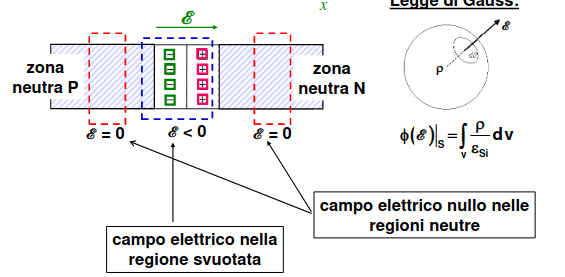
\includegraphics[width=0.5\linewidth]{imgs/giunzione-svuotata}
    \caption{Rappresentazioni regione svuotata e zona neutra}
    \label{fig:reg_svuot_neutr}
\end{figure}

\subsubsection{Regione svuotata: potenziale V}
\begin{equation}
    \epsilon = -\frac{dV}{dx}
\end{equation}
Si crea una caduta di potenziale agli estremi della regione svuotata.
Se si prende come 0 l'anodo(P) si ottiene un risultato positivo di tensione $V=V_{bi}$(potenziale di built-in).

\begin{figure}[H]
    \centering
    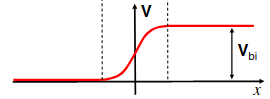
\includegraphics[width=0.4\linewidth]{/home/dmo/git/appunti-latex-2021-2022/APPLICAZIONI INDUSTRIALI ELETTRICHE ED ELETTRONICA/imgs/tensione-built-in}
    \caption{Tensione built-in}
    \label{fig:built-in}
\end{figure}


\subsection{Diodo polarizzato in diretta ($V_D>0$)}
\begin{figure}[H]
    \centering
    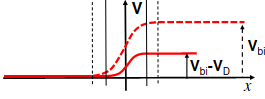
\includegraphics[width=0.4\linewidth]{imgs/polarizzato-direttamente}
    \caption{Diodo polarizzato direttamente}
    \label{fig:polarizzato-direttamente}
\end{figure}

Si abbassa la barriera che inpediva il fluire della corrente.
\subsubsection{Caratteristiche $I_D(V_D)$ in diretta}
\begin{equation}
    I_D = I_S(e^{\frac{V_D}{V_T} - 1}) \cong I_{S}e^{\frac{V_D}{V_T}}
\end{equation}

Dove la tensione del diodo della tensione termica($V_D >> V_T$).

Tensione termica:
\begin{equation*}
    V_T = \frac{kT}{q}
\end{equation*}
La tensione termica con temperatura $300K$ è $25,6mV$.

La $I_S$ è la corrente inversa di saturazione.

La tensione del diodo si approssima a circa $V_D = \cong 0,7V$

\subsection{Diodo polarizzato in inversa e breakdown ($V_D < 0$)}

Essendo una tensione negativa, la "barriera" che inpediva il fluire della corrente viene aumentata.

\subsubsection{Breakdown a valanga}
Il diodo il polarizzazione inversa, regge la tensione fin al punto di breakdown senza far passare la corrente,
dopodichè cede, distruggendosi.

\begin{figure}[H]
    \centering
    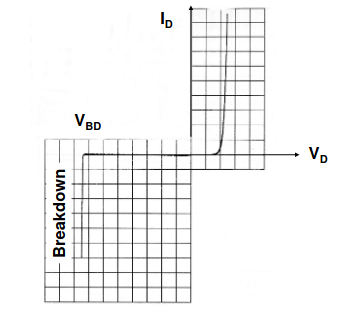
\includegraphics[width=0.3\linewidth]{imgs/breakdown}
    \caption{comportamento reale del diodo}
    \label{fig:breakdown}
\end{figure}

\subsection{Applicazione del diodo}
\subsubsection{Raddrizzatore}
\begin{figure}[H]
    \centering
    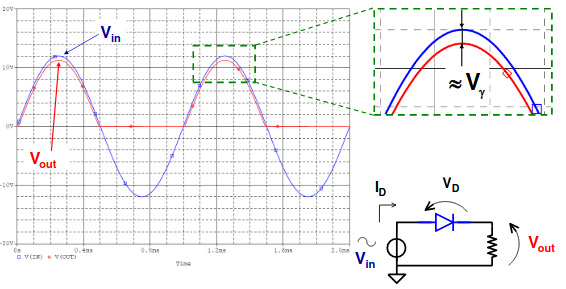
\includegraphics[width=0.7\linewidth]{imgs/radrizzatore}
    \caption{radrizzatore}
    \label{fig:radrizzatore}

\end{figure}
Solitamente si utilizzano i diodi zener che hanno una tensione di breakdown enorme se si vogliono usare come
radrizzatori di un segnale alternato.

\subsubsection{Rilevatori di picco}
\begin{figure}[H]
    \centering
    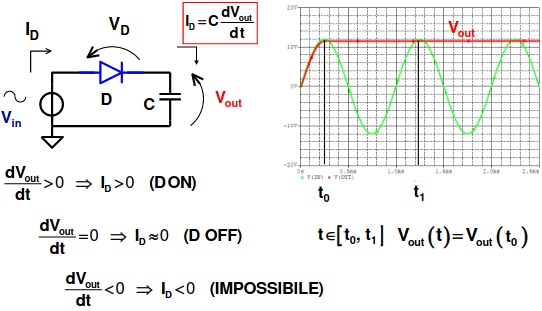
\includegraphics[width=0.8\linewidth]{imgs/rilevatore-di-picco}
    \caption{rilevatore di picco}
    \label{fig:rilevatore-di-picco}
\end{figure}

\subsection{Capacità del diodo e modello circuitale}
La capacità per la tensione del diodo($0.7V$):
\begin{equation}
    Q_J(V_D) = K_j \sqrt {V_{bi} - V_D}
\end{equation}

\begin{figure}[H]
    \centering
    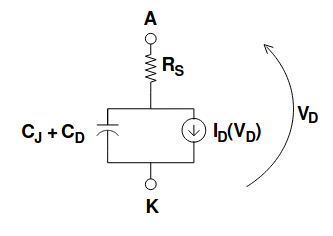
\includegraphics[width=0.5\linewidth]{imgs/modello-del-diodo}
    \caption{modello del diodo}
    \label{fig:modello-del-diodo}
\end{figure}


















